%%%%%%%%%%%%%%%%%%%%%%%%%%%%%%%%%%%%%%%%%
% Beamer Presentation
% LaTeX Template
% Version 2.0 (March 8, 2022)
%
% This template originates from:
% https://www.LaTeXTemplates.com
%
% Author:
% Vel (vel@latextemplates.com)
%
% License:
% CC BY-NC-SA 4.0 (https://creativecommons.org/licenses/by-nc-sa/4.0/)
%
%%%%%%%%%%%%%%%%%%%%%%%%%%%%%%%%%%%%%%%%%

%----------------------------------------------------------------------------------------
%	PACKAGES AND OTHER DOCUMENT CONFIGURATIONS
%----------------------------------------------------------------------------------------

\documentclass[handout, % remove this to include pauses
	11pt, % Set the default font size, options include: 8pt, 9pt, 10pt, 11pt, 12pt, 14pt, 17pt, 20pt
	%t, % Uncomment to vertically align all slide content to the top of the slide, rather than the default centered
	%aspectratio=169, % Uncomment to set the aspect ratio to a 16:9 ratio which matches the aspect ratio of 1080p and 4K screens and projectors
]{beamer}

% \graphicspath{{Images/}{./}} % Specifies where to look for included images (trailing slash required)

% \usepackage{nirav}
\usepackage{todo}
\usepackage{booktabs} % Allows the use of \toprule, \midrule and \bottomrule for better rules in tables

%----------------------------------------------------------------------------------------
%	SELECT LAYOUT THEME
%----------------------------------------------------------------------------------------

% Beamer comes with a number of default layout themes which change the colors and layouts of slides. Below is a list of all themes available, uncomment each in turn to see what they look like.

%\usetheme{default}
%\usetheme{AnnArbor}
%\usetheme{Antibes}
%\usetheme{Bergen}
%\usetheme{Berkeley}
%\usetheme{Berlin}
%\usetheme{Boadilla}
%\usetheme{CambridgeUS}
%\usetheme{Copenhagen}
%\usetheme{Darmstadt}
%\usetheme{Dresden}
%\usetheme{Frankfurt}
%\usetheme{Goettingen}
%\usetheme{Hannover}
%\usetheme{Ilmenau}
%\usetheme{JuanLesPins}
%\usetheme{Luebeck}
\usetheme{Madrid}
%\usetheme{Malmoe}
%\usetheme{Marburg}
%\usetheme{Montpellier}
%\usetheme{PaloAlto}
%\usetheme{Pittsburgh}
%\usetheme{Rochester}
%\usetheme{Singapore}
%\usetheme{Szeged}
%\usetheme{Warsaw}

%----------------------------------------------------------------------------------------
%	SELECT COLOR THEME
%----------------------------------------------------------------------------------------

% Beamer comes with a number of color themes that can be applied to any layout theme to change its colors. Uncomment each of these in turn to see how they change the colors of your selected layout theme.

%\usecolortheme{albatross}
%\usecolortheme{beaver}
%\usecolortheme{beetle}
%\usecolortheme{crane}
%\usecolortheme{dolphin}
%\usecolortheme{dove}
%\usecolortheme{fly}
%\usecolortheme{lily}
%\usecolortheme{monarca}
%\usecolortheme{seagull}
%\usecolortheme{seahorse}
%\usecolortheme{spruce}
%\usecolortheme{whale}
%\usecolortheme{wolverine}

%----------------------------------------------------------------------------------------
%	SELECT FONT THEME & FONTS
%----------------------------------------------------------------------------------------

% Beamer comes with several font themes to easily change the fonts used in various parts of the presentation. Review the comments beside each one to decide if you would like to use it. Note that additional options can be specified for several of these font themes, consult the beamer documentation for more information.

\usefonttheme{default} % Typeset using the default sans serif font
%\usefonttheme{serif} % Typeset using the default serif font (make sure a sans font isn't being set as the default font if you use this option!)
%\usefonttheme{structurebold} % Typeset important structure text (titles, headlines, footlines, sidebar, etc) in bold
%\usefonttheme{structureitalicserif} % Typeset important structure text (titles, headlines, footlines, sidebar, etc) in italic serif
%\usefonttheme{structuresmallcapsserif} % Typeset important structure text (titles, headlines, footlines, sidebar, etc) in small caps serif

%------------------------------------------------

%\usepackage{mathptmx} % Use the Times font for serif text
\usepackage{palatino} % Use the Palatino font for serif text

%\usepackage{helvet} % Use the Helvetica font for sans serif text
\usepackage[default]{opensans} % Use the Open Sans font for sans serif text
%\usepackage[default]{FiraSans} % Use the Fira Sans font for sans serif text
%\usepackage[default]{lato} % Use the Lato font for sans serif text

%----------------------------------------------------------------------------------------
%	SELECT INNER THEME
%----------------------------------------------------------------------------------------

% Inner themes change the styling of internal slide elements, for example: bullet points, blocks, bibliography entries, title pages, theorems, etc. Uncomment each theme in turn to see what changes it makes to your presentation.

%\useinnertheme{default}
\useinnertheme{circles}
%\useinnertheme{rectangles}
%\useinnertheme{rounded}
%\useinnertheme{inmargin}

%----------------------------------------------------------------------------------------
%	SELECT OUTER THEME
%----------------------------------------------------------------------------------------

% Outer themes change the overall layout of slides, such as: header and footer lines, sidebars and slide titles. Uncomment each theme in turn to see what changes it makes to your presentation.

%\useoutertheme{default}
%\useoutertheme{infolines}
%\useoutertheme{miniframes}
%\useoutertheme{smoothbars}
%\useoutertheme{sidebar}
%\useoutertheme{split}
%\useoutertheme{shadow}
%\useoutertheme{tree}
%\useoutertheme{smoothtree}

%\setbeamertemplate{footline} % Uncomment this line to remove the footer line in all slides
%\setbeamertemplate{footline}[page number] % Uncomment this line to replace the footer line in all slides with a simple slide count

%\setbeamertemplate{navigation symbols}{} % Uncomment this line to remove the navigation symbols from the bottom of all slides

%----------------------------------------------------------------------------------------
%	PRESENTATION INFORMATION
%----------------------------------------------------------------------------------------

\title[KSP Week 3 Presentation]{KSP Week 3 Presentation} % The short title in the optional parameter appears at the bottom of every slide, the full title in the main parameter is only on the title page

% \subtitle{MA105 Tutorial Sheet - 1} % Presentation subtitle, remove this command if a subtitle isn't required

\author[Nirav]{Nirav Bhattad} % Presenter name(s), the optional parameter can contain a shortened version to appear on the bottom of every slide, while the main parameter will appear on the title slide

% \institute[UC]{IIT Bombay \\ \smallskip \textit{22b0967@iitb.ac.in}} % Your institution, the optional parameter can be used for the institution shorthand and will appear on the bottom of every slide after author names, while the required parameter is used on the title slide and can include your email address or additional information on separate lines

\date[\today]{KSP Week 3 Presentation} % Presentation date or conference/meeting name, the optional parameter can contain a shortened version to appear on the bottom of every slide, while the required parameter value is output to the title slide

%----------------------------------------------------------------------------------------
\setbeamertemplate{navigation symbols}{}
\begin{document}

%----------------------------------------------------------------------------------------
%	TITLE SLIDE
%----------------------------------------------------------------------------------------

\begin{frame}
	\titlepage % Output the title slide, automatically created using the text entered in the PRESENTATION INFORMATION block above
\end{frame}

%----------------------------------------------------------------------------------------
%	TABLE OF CONTENTS SLIDE
%----------------------------------------------------------------------------------------

\section{Finding Our Way in the Sky}
\begin{frame}
    \frametitle{Finding Our Way in the Sky}
    \begin{itemize}
        \item Radio astronomers use the celestial coordinate system to locate objects in the sky.
        \item The system is similar to the latitude and longitude system used on Earth.
        \item Key coordinates:
            \begin{itemize}
                \item \textbf{Right Ascension} (RA - $\alpha$) - analogous to longitude, measured in hours, minutes, and seconds.
                \item \textbf{Declination} (Dec - $\delta$)- analogous to latitude, measured in degrees, arcminutes, and arcseconds.
            \end{itemize}
        \item Radio telescopes can be precisely aimed using these coordinates.
        \item Seconds of Arc $ = 15 \cos (\delta) \times \text{Seconds of RA}$
    \end{itemize}
\end{frame}

\begin{frame}
    \frametitle{Celestial Coordinate System}
    \begin{figure}
        \centering
        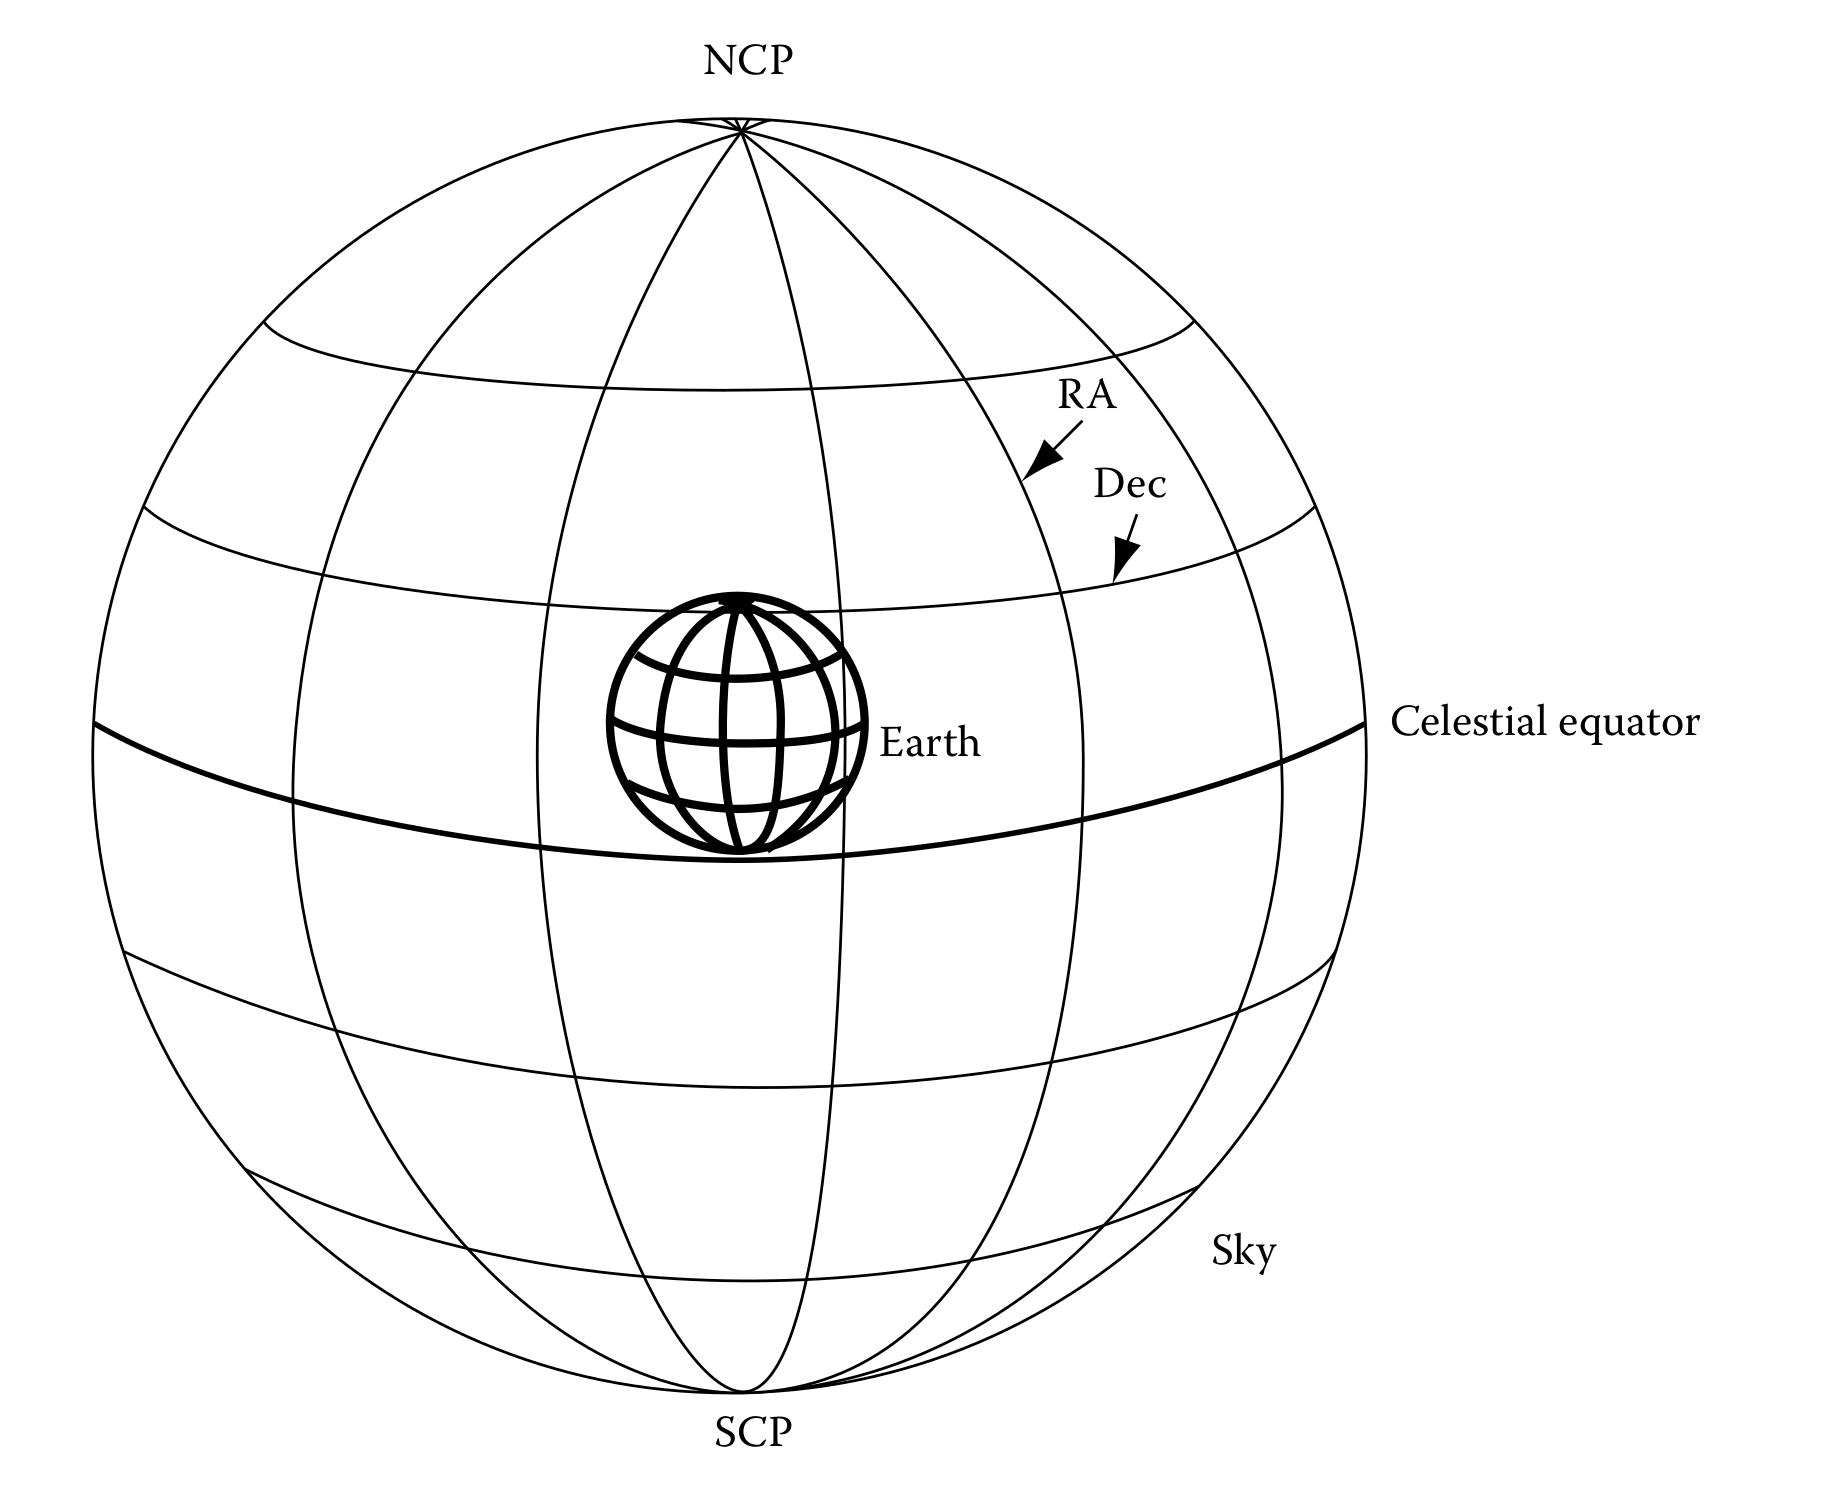
\includegraphics[width=0.6\textwidth]{Images/celestial_coordinate_system.png}
        \caption{Celestial coordinate system}
        \label{fig:celestial_coordinates}
    \end{figure}
\end{frame}

\begin{frame}
    \frametitle{Observer-Centered Definitions}
    \begin{itemize}
        \item \textbf{Horizon:} The circle where the sky meets the Earth.
        \item \textbf{Zenith:} The point directly above the observer.
        \item \textbf{Altitude or Elevation:} Angular height of an object above your horizon at any given moment
        \item \textbf{Azimuth:} The angular position of an object along the horizon relative to due north.
        \item \textbf{Meridian:} The line that goes from the north to the south pole.
        \item \textbf{Transit:} The moment when an object crosses the meridian.
        \item \textbf{Hour Angle:} The angular distance between the meridian and the object.
    \end{itemize}

    Azimuth and Altitude make a pair of angles that completely define an object’s position in the sky \textit{relative to the observer,} whereas RA and Dec are \textit{absolute} coordinates.
\end{frame}

\begin{frame}
    \frametitle{Sky Coordinates Example}
    \begin{figure}
        \centering
        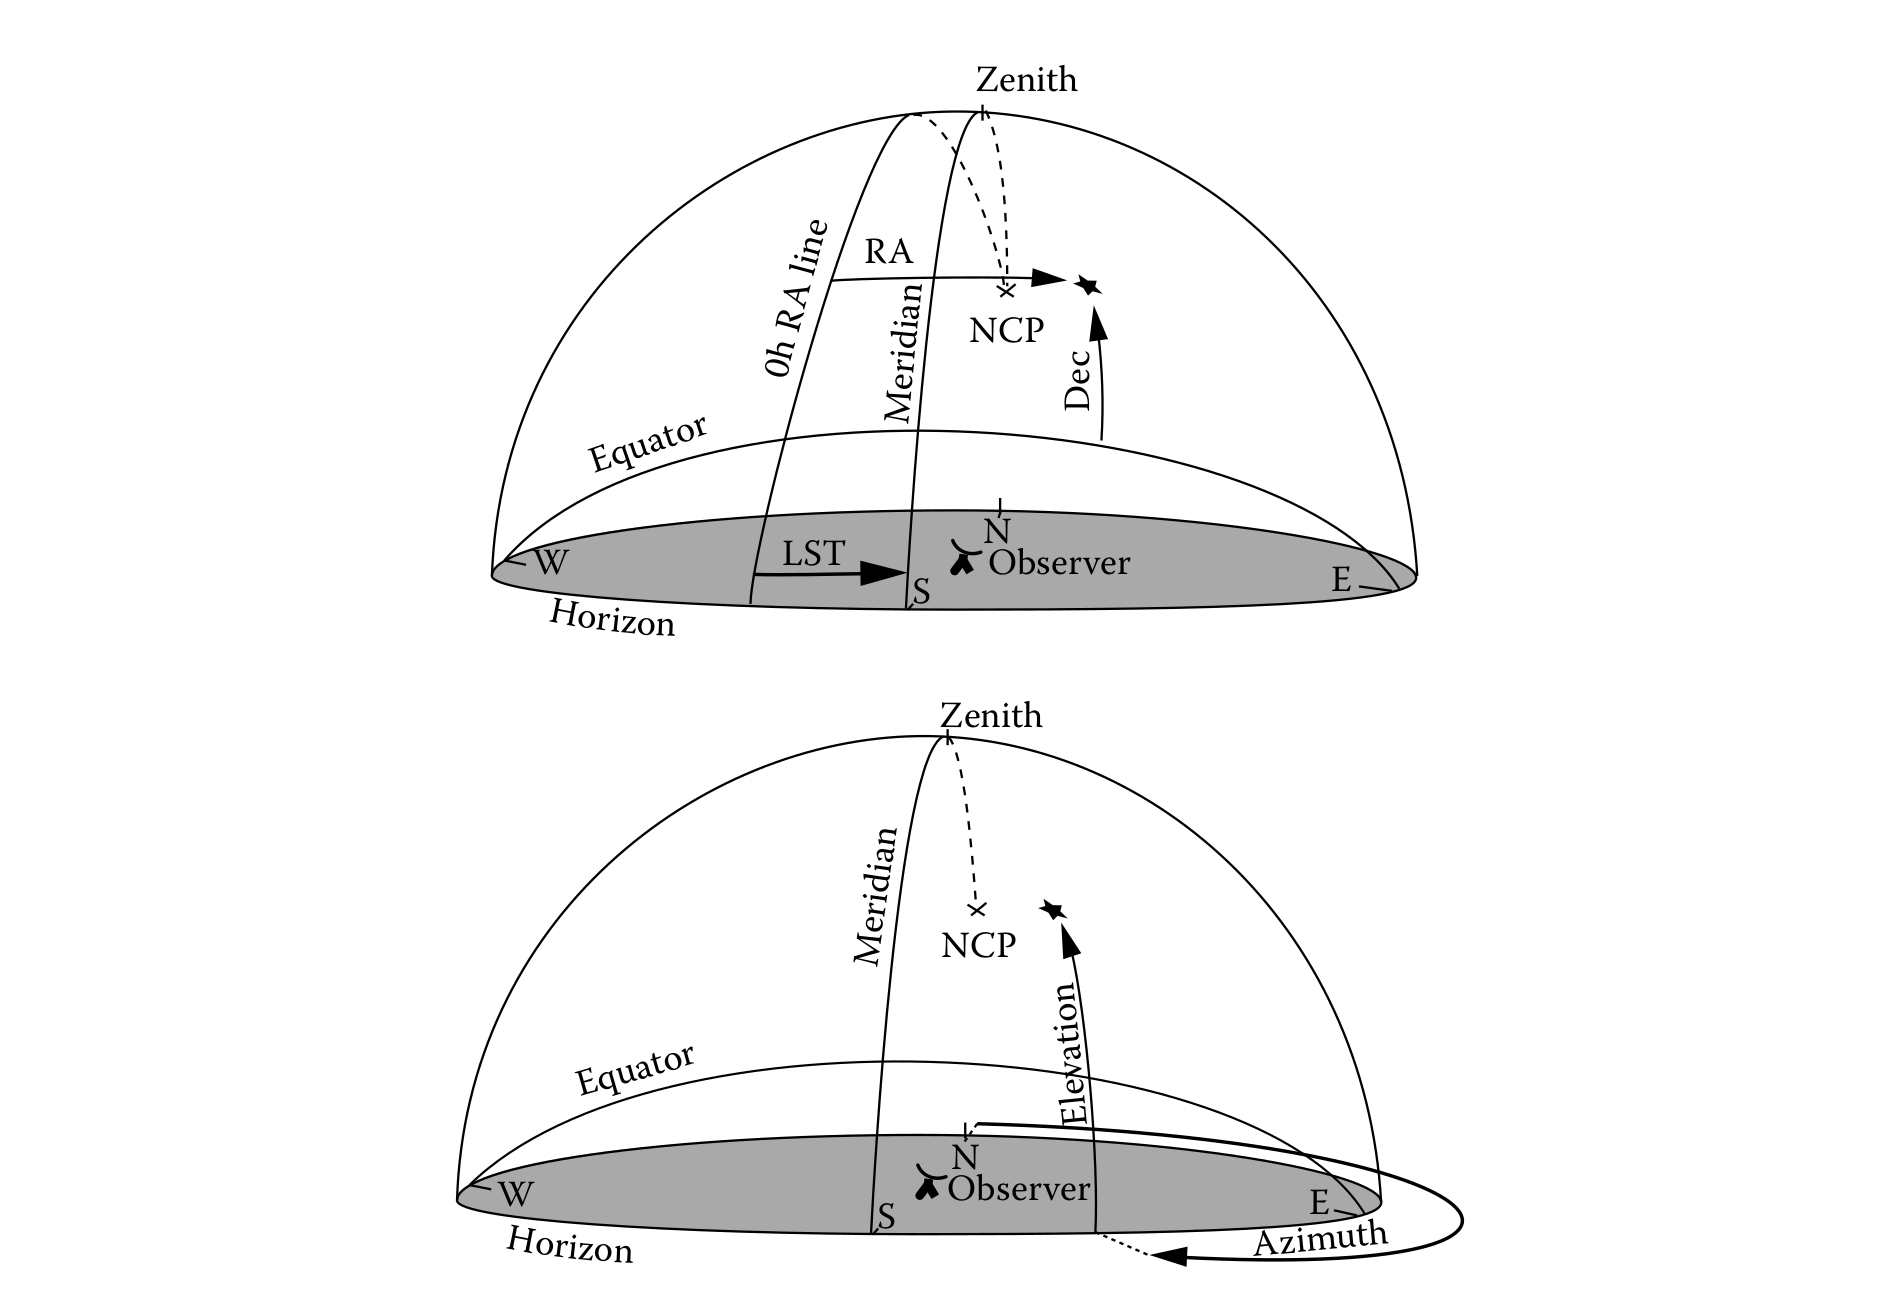
\includegraphics[width=0.6\textwidth]{Images/sky_coordinates_example.png}
        \caption{Depiction of sky coordinates as viewed by the observer (top) and observer-centered coordinates (bottom)}
        \label{fig:sky_coordinates_example}
    \end{figure}
\end{frame}

\begin{frame}
    \frametitle{Apparent Sizes}
    \begin{itemize}
        \item The apparent size of an object in the sky depends on the distance to the object.
        % Solid Angle 
        \item The solid angle subtended by an object is the angle that the object appears to occupy in the sky.
        \item Solid angle is measured in steradians.
        % formula
        \item The solid angle $\Omega$ subtended by an object is given by 
        \[
            \Omega = \frac{A}{r^2} 
        \]
        where $A$ is the area of the object and $r$ is the distance to the object.
        \item The solid angle of a sphere with radius $r$ is $4\pi$ steradians.
    \end{itemize}
\end{frame}


\section{Basic Structure of a Traditional Radio Telescope}
\begin{frame}
    \frametitle{Basic Structure of a Traditional Radio Telescope}
    \begin{itemize}
        \item The primary components of a radio telescope:
            \begin{itemize}
                \item Antenna - collects radio waves.
                \item Receiver - amplifies the weak signals collected by the antenna.
                \item Amplifier - further boosts the signal strength.
                \item Detector - converts the radio signals into a form that can be recorded and analyzed.
                \item Data Recorder - stores the signal data for further processing.
            \end{itemize}
        \item The dish shape of the antenna helps focus the radio waves onto the receiver.
        \item Modern radio telescopes often use arrays of antennas to increase resolution and sensitivity.
    \end{itemize}
\end{frame}

% \begin{frame}
%     \begin{figure}
%         \centering
%         \includegraphics[width=0.6\textwidth]{radio_telescope_structure.jpg}
%         \caption{Basic structure of a traditional radio telescope}
%         \label{fig:radio_telescope_structure}
%     \end{figure}
% \end{frame}

\section{Basic Structure of a Traditional Radio Telescope}
\begin{frame}
    \frametitle{Basic Structure of a Traditional Radio Telescope}
    \begin{itemize}
        \item A traditional radio telescope has five main parts: parabolic reflector, mount, feeds, receivers, and computer.
        \item \textbf{Parabolic Reflector}:
            \begin{itemize}
                \item Collects and focuses radio waves.
                \item Sensitivity depends on the dish's diameter.
                \item Example: The Arecibo telescope (305 meters in diameter).
            \end{itemize}
        \item \textbf{Mount}:
            \begin{itemize}
                \item Holds and moves the dish.
                \item Altitude-Azimuth mounts are commonly used.
            \end{itemize}
        \item \textbf{Feeds and Receivers}:
            \begin{itemize}
                \item Feeds convert EM waves to signals.
                \item Receivers process and amplify signals.
            \end{itemize}
        \item \textbf{Computer}:
            \begin{itemize}
                \item Stores and analyzes the digital signal.
            \end{itemize}
    \end{itemize}
\end{frame}

\begin{frame}
    \frametitle{Basic Structure of a Traditional Radio Telescope}
    \begin{figure}
        \centering
        \includegraphics[width=0.6\textwidth]{Images/radio_telescope_structure.png}
        \caption{Basic structure of a traditional radio telescope}
        \label{fig:radio_telescope_structure}
    \end{figure}
\end{frame}

\begin{frame}
    \frametitle{Measures of the Amount of Radiation}
    \begin{itemize}
        \item \textbf{Total Energy Emitted} - The total energy emitted by an object.
        \item \textbf{Luminosity} ($L$) - The total energy emitted by an object per unit time in all directions.
        \item \textbf{Flux} ($F$) - The energy received per unit time per unit area.
        \item \textbf{Flux Density} ($F_{\nu}$) - The flux per unit frequency interval.
        \item \textbf{Intensity} ($I_{\nu}$) - The flux density per unit solid angle.
    \end{itemize}
\end{frame}

% \begin{frame}
%     \frametitle{Blackbody Radiation}

\end{document} 